\section{Graphics}
\subsection{Introduction to Graphs in Stata}

This module will introduce some basic graphs in Stata 12, including histograms, boxplots, scatterplots, and scatterplot matrices.

Let's use the \lstinline{auto} data file for making some graphs.

\begin{lstlisting}
sysuse auto.dta
\end{lstlisting}

The \lstinline{histogram} command can be used to make a simple histogram of \textit{mpg}

\begin{lstlisting}
histogram mpg
\end{lstlisting}

\begin{figure}[!htbp]
\centering
\includegraphics[width=0.4\textwidth]{mod311.pdf}
\includegraphics[width=0.4\textwidth]{mod312.pdf}
\caption{\lstinline{histogram}, the right graph with option \lstinline{discrete}\label{histogram}}
\end{figure}

If you are creating a histogram for a categorical variable such as rep78,  you can add the option \lstinline{discrete}. As you can see below, when you specify this option, the midpoint of each bin labels the respective bar.

\begin{lstlisting}
hist rep78, percent discrete
\end{lstlisting}

The \lstinline{graph} \lstinline{box} command can be used to produce a boxplot which can help you examine the distribution of \textit{mpg}. If \textit{mpg} were normally distributed, the line (the median) would be in the middle of the box (the 25th and 75th percentiles, Q1 and Q3) and the ends of the whiskers (the upper and lower adjacent values, which are the most extreme values within Q3+1.5(Q3-Q1) and Q1-1.5*(Q3-Q1), respectively) would be equidistant from the box. The boxplot for \textit{mpg} shows positive skew. The median is pulled to the low end of the box.

\begin{lstlisting}
graph box mpg
\end{lstlisting}

\begin{figure}[!htbp]
\centering
\includegraphics[width=0.4\textwidth]{mod313.pdf}
\includegraphics[width=0.4\textwidth]{mod314.pdf}
\caption{\lstinline{graph box}, the right graph with option \lstinline{by}\label{box}}
\end{figure}

The boxplot can be done separately for foreign and domestic cars using the\lstinline{ by( )} or \lstinline{over( )} option.

\begin{lstlisting}
graph box mpg, by(foreign)
\end{lstlisting}

\begin{lstlisting}
graph box mpg, over(foreign)
\end{lstlisting}

As you can see in the graph above, there are a pair of outliers in the box plots produced. These can be removed from the box plot using the \lstinline{noout} command in Stata.

\begin{lstlisting}
graph box mpg, over(foreign) noout
\end{lstlisting}

\begin{figure}[!htbp]
\centering
\includegraphics[width=0.4\textwidth]{mod315.pdf}
\includegraphics[width=0.4\textwidth]{mod316.pdf}
\caption{\lstinline{graph box} with \lstinline{over}, the right graph with option \lstinline{noout}\label{box2}}
\end{figure}

The graph no longer includes the outlying values. Stata also includes a message at the bottom of the graph noting that outside values were excluded.

Stata can also produce pie charts.

\begin{lstlisting}
graph pie, over(rep78) plabel(_all name) title("Repair Record 1978")
\end{lstlisting}

\begin{center}
\includegraphics[width=0.4\textwidth]{mod317.pdf}
\end{center}

The \lstinline{graph pie} command with the \lstinline{over} option creates a pie chart representing the frequency of each group or value of \textit{rep78}. The \lstinline{plabel} option places the value labels for \textit{rep78} inside each slice of the pie chart.

A two way scatter plot can be used to show the relationship between \textit{mpg} and \textit{weight}. As we would expect, there is a negative relationship between \textit{mpg} and \textit{weight}.

\begin{lstlisting}
graph twoway scatter mpg weight
\end{lstlisting}

\begin{figure}[!htbp]
\centering
\includegraphics[width=0.4\textwidth]{mod318.pdf}
\includegraphics[width=0.4\textwidth]{mod319.pdf}
\caption{\lstinline{twoway graph}, the left graph is \lstinline{scatter} and the right is \lstinline{lfit}\label{twoway}}
\end{figure}

Note that you can save typing like this

\begin{lstlisting}
twoway scatter mpg weight
\end{lstlisting}

We can show the regression line predicting mpg from weight like this.

\begin{lstlisting}
twoway lfit mpg weight
\end{lstlisting}


We can combine these graphs like shown below.

\begin{lstlisting}
twoway (scatter mpg weight) (lfit mpg weight)
\end{lstlisting}

\begin{center}
\includegraphics[width=0.4\textwidth]{mod3110.pdf}
\end{center}

We can add labels to the points labeling them by make as shown below. Note that mlabel is an option on the scatter command.

\begin{lstlisting}
twoway (scatter mpg weight, mlabel(make) ) (lfit mpg weight)
\end{lstlisting}


The marker label position can be changed using the \lstinline{mlabangle( )} option.

\begin{lstlisting}
twoway (scatter mpg weight, mlabel(make) mlabangle(45)) (lfit mpg weight)
\end{lstlisting}

\begin{figure}[!h]
\centering
\includegraphics[width=0.4\textwidth]{mod3111.pdf}
\includegraphics[width=0.4\textwidth]{mod3112.pdf}
\caption{\lstinline{twoway graph mlabel}, the right graph with option \lstinline{mlabangle}\label{twowayx}}
\end{figure}


We can combine separate graphs for foreign and domestic cars as shown below, and we have requested confidence bands around the predicted values by using \lstinline{lfitci} in place of \lstinline{lfit} .  Note that the \lstinline{by} option is at the end of the command.

\begin{lstlisting}
twoway (scatter mpg weight) (lfitci mpg weight), by(foreign)
\end{lstlisting}

You can request a scatter plot matrix with the \lstinline{graph matrix} command. Here we examine the relationships among \textit{mpg}, \textit{weight} and \textit{price}.

\begin{lstlisting}
graph matrix mpg weight price
\end{lstlisting}

\begin{figure}[!htbp]
\centering
\includegraphics[width=0.4\textwidth]{mod3113.pdf}
\includegraphics[width=0.4\textwidth]{mod3114.pdf}
\caption{\lstinline{twoway graph with lfitci and graph matrix}\label{twowayxx}}
\end{figure}


\subsection{Graphics: Overview of Twoway Plots}
This module shows examples of the different kinds of graphs that can be created with the \lstinline{graph twoway} command.  This is illustrated by showing the command and the resulting graph.  For more information, see the \href{http://www.stata.com/help.cgi?graph}{Stata Graphics Manual} available over the web and from within Stata by typing \lstinline{help graph}, and in particular the section on \href{http://www.stata.com/help.cgi?scatter}{Two Way Scatterplots}.

\textbf{Basic twoway scatterplot V.S. Line Plot}
\begin{lstlisting}
sysuse sp500
graph twoway scatter close date // the left graph
graph twoway line close date    // the right graph
\end{lstlisting}
\begin{center}
\includegraphics[width=0.4\textwidth]{mod321.pdf}
\includegraphics[width=0.4\textwidth]{mod322.pdf}
\end{center}

\textbf{Connected Line Plot}
\begin{lstlisting}
graph twoway connected close date
\end{lstlisting}


\textbf{Immediate scatterplot}
\begin{lstlisting}
graph twoway scatteri ///
  965.8    15239 (3) "Low   965.8" ///
  1373.73  15005 (3) "High 1373.73" , msymbol(i)
\end{lstlisting}

\textbf{Scatterplot and Immediate Scatterplot}
\begin{lstlisting}
graph twoway ///
  (scatter close date) ///
  (scatteri  965.8  15239 (3) "Low, 9/21, 965.8" ///
            1373.7  15005 (3) "High, 1/30, 1373.7", msymbol(i) )
\end{lstlisting}
\begin{center}
\includegraphics[width=0.33\textwidth]{mod323.pdf}\hfil
\includegraphics[width=0.33\textwidth]{mod324.pdf}\hfil
\includegraphics[width=0.33\textwidth]{mod325.pdf}\\
Left graph is twoway scatter plot; the center is the immediate scatter plot; the right is the combination of the two.
\end{center}

\textbf{Area Graph}
\begin{lstlisting}
drop if _n > 57
graph twoway area close date, sort
\end{lstlisting}

\textbf{Bar plot}
\begin{lstlisting}
graph twoway bar close date
\end{lstlisting}

\textbf{Spike plot}
\begin{lstlisting}
graph twoway spike close date
\end{lstlisting}

\textbf{Dropline plot}
\begin{lstlisting}
graph twoway dropline close date
\end{lstlisting}

\begin{center}
\includegraphics[width=0.40\textwidth]{mod326.pdf}
\includegraphics[width=0.40\textwidth]{mod327.pdf}\\
\textbf{Notes:} The left plot is \lstinline{area} plot; the right one is \lstinline{bar} plot.\\
\includegraphics[width=0.40\textwidth]{mod328.pdf}
\includegraphics[width=0.40\textwidth]{mod329.pdf}\\
\textbf{Notes:} The left plot is \lstinline{spike} plot; the right one is \lstinline{dropline} plot.\\
\end{center}

\textbf{Dot plot}
\begin{lstlisting}
graph twoway dot change date
\end{lstlisting}

\textbf{Range plot with area shading}
\begin{lstlisting}
graph twoway rarea high low date
\end{lstlisting}

\textbf{Range plot with bars}
\begin{lstlisting}
graph twoway rbar high low date
\end{lstlisting}

\begin{center}
\includegraphics[width=0.33\textwidth]{mod3210.pdf}
\includegraphics[width=0.33\textwidth]{mod3211.pdf}
\includegraphics[width=0.33\textwidth]{mod3212.pdf}\\
Left graph is \lstinline{dot} plot; the center is \lstinline{rarea} plot; the right is \lstinline{rbar} plot.
\end{center}

\textbf{Range plot with spikes}
\begin{lstlisting}
graph twoway rspike high low date
\end{lstlisting}

\textbf{Range plot with capped spikes}
\begin{lstlisting}
graph twoway rcap high low date
\end{lstlisting}

\textbf{Range plot with spikes capped with symbols}
\begin{lstlisting}
graph twoway rcapsym high low date
\end{lstlisting}

\begin{center}
\includegraphics[width=0.33\textwidth]{mod3213.pdf}
\includegraphics[width=0.33\textwidth]{mod3214.pdf}
\includegraphics[width=0.33\textwidth]{mod3215.pdf}\\
Left graph is \lstinline{rspike} plot; the center is \lstinline{rcap} plot; the right is \lstinline{rcapsym} plot.
\end{center}

\textbf{Range plot with markers}
\begin{lstlisting}
graph twoway rscatter high low date
\end{lstlisting}

\textbf{Range plot with lines}
\begin{lstlisting}
graph twoway rline high low date
\end{lstlisting}

\textbf{Range plot with lines and markers}
\begin{lstlisting}
graph twoway rconnected high low date
\end{lstlisting}

\begin{center}
\includegraphics[width=0.33\textwidth]{mod3216.pdf}
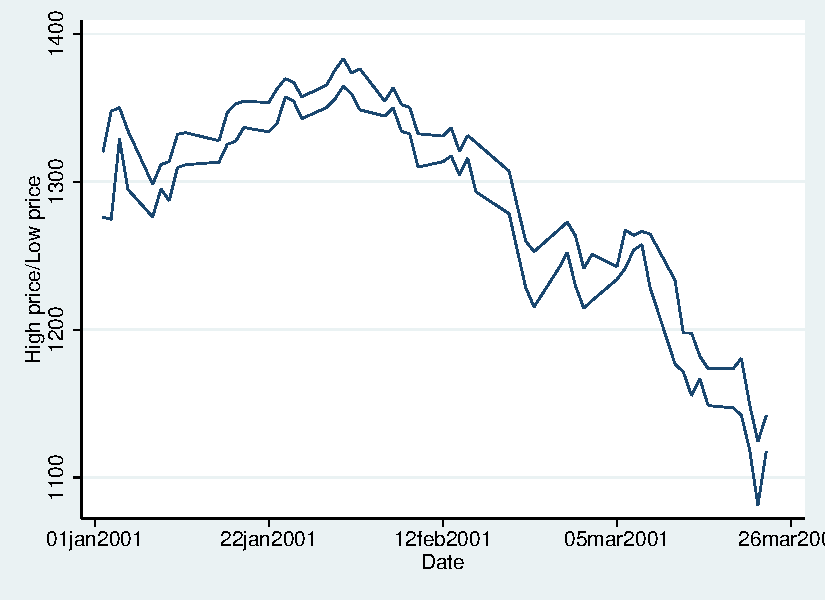
\includegraphics[width=0.33\textwidth]{mod3217.pdf}
\includegraphics[width=0.33\textwidth]{mod3218.pdf}\\
Left graph is \lstinline{rscatter} plot; the center is \lstinline{rline} plot; the right is \lstinline{rconnected} plot.
\end{center}

% new dataset
\textbf{Median band line plot}
\begin{lstlisting}
use "http://www.ats.ucla.edu/stat/stata/notes/hsb2.dta", clear
graph twoway mband read write
\end{lstlisting}

\textbf{Spline line plot}
\begin{lstlisting}
graph twoway mspline read write
\end{lstlisting}

\textbf{LOWESS line plot}
\begin{lstlisting}
graph twoway lowess read write
\end{lstlisting}

\begin{center}
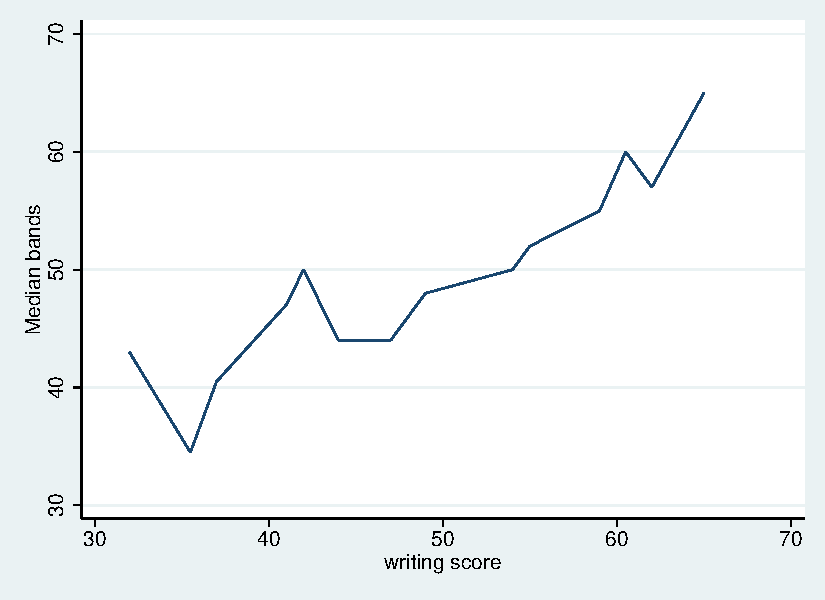
\includegraphics[width=0.33\textwidth]{mod3219.pdf}
\includegraphics[width=0.33\textwidth]{mod3220.pdf}
\includegraphics[width=0.33\textwidth]{mod3221.pdf}\\
Left graph is \lstinline{mband} plot; the center is \lstinline{mspline} plot; the right is \lstinline{lowess} plot.
\end{center}


\textbf{Linear prediction plot}
\begin{lstlisting}
graph twoway lfit read write
\end{lstlisting}

\textbf{Quadratic prediction plot}
\begin{lstlisting}
graph twoway qfit read write
\end{lstlisting}

\textbf{Fractional polynomial plot}
\begin{lstlisting}
graph twoway fpfit read write
\end{lstlisting}

\begin{center}
\includegraphics[width=0.33\textwidth]{mod3222.pdf}
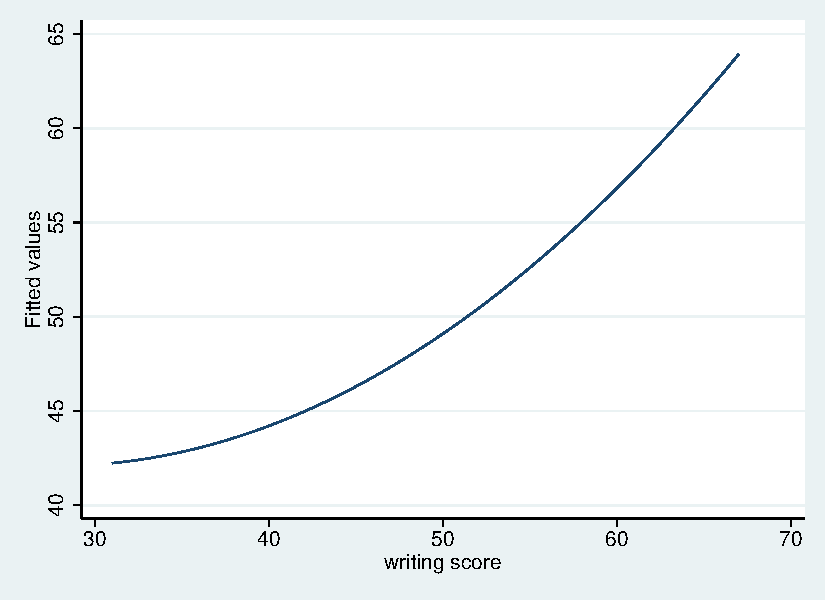
\includegraphics[width=0.33\textwidth]{mod3223.pdf}
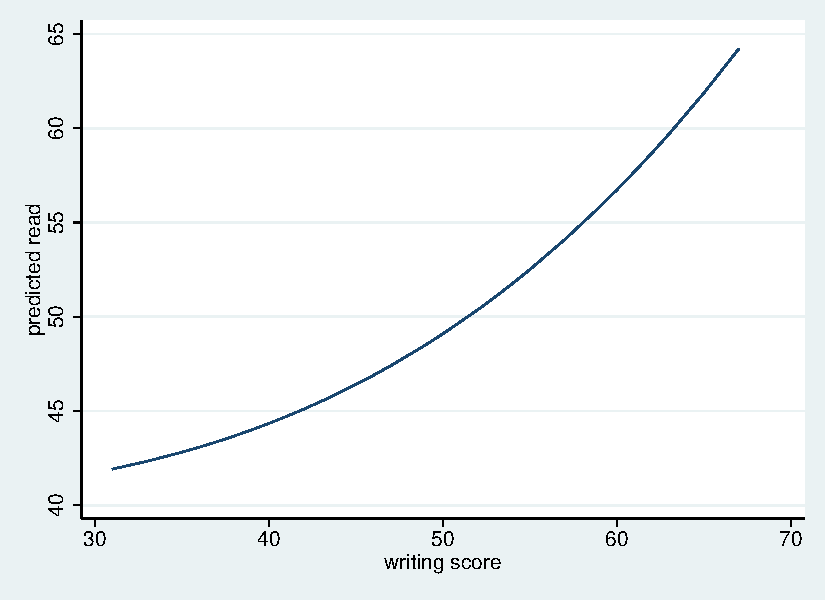
\includegraphics[width=0.33\textwidth]{mod3224.pdf}\\
Left graph is \lstinline{lfit} plot; the center is \lstinline{qfit} plot; the right is \lstinline{fpfit} plot.
\end{center}



\textbf{Linear prediction plot with confidence intervals}
\begin{lstlisting}
graph twoway lfitci read write
\end{lstlisting}

\textbf{Quadratic plot with confidence intervals}
\begin{lstlisting}
graph twoway qfitci read write
\end{lstlisting}

\textbf{Fractional polynomial plot with CIs}
\begin{lstlisting}
graph twoway fpfitci read write
\end{lstlisting}

\begin{center}
\includegraphics[width=0.33\textwidth]{mod3225.pdf}
\includegraphics[width=0.33\textwidth]{mod3226.pdf}
\includegraphics[width=0.33\textwidth]{mod3227.pdf}\\
Left graph is \lstinline{lfitci} plot; the center is \lstinline{qfitci} plot; the right is \lstinline{fpfitci} plot.
\end{center}



\textbf{Histogram}
\begin{lstlisting}
graph twoway histogram read
\end{lstlisting}

\textbf{Kernel density plot}
\begin{lstlisting}
graph twoway kdensity read
\end{lstlisting}

\textbf{Function plot}
\begin{lstlisting}
graph twoway function y=normalden(x), range(-4 4)
\end{lstlisting}
\begin{center}
\includegraphics[width=0.33\textwidth]{mod3228.pdf}
\includegraphics[width=0.33\textwidth]{mod3229.pdf}
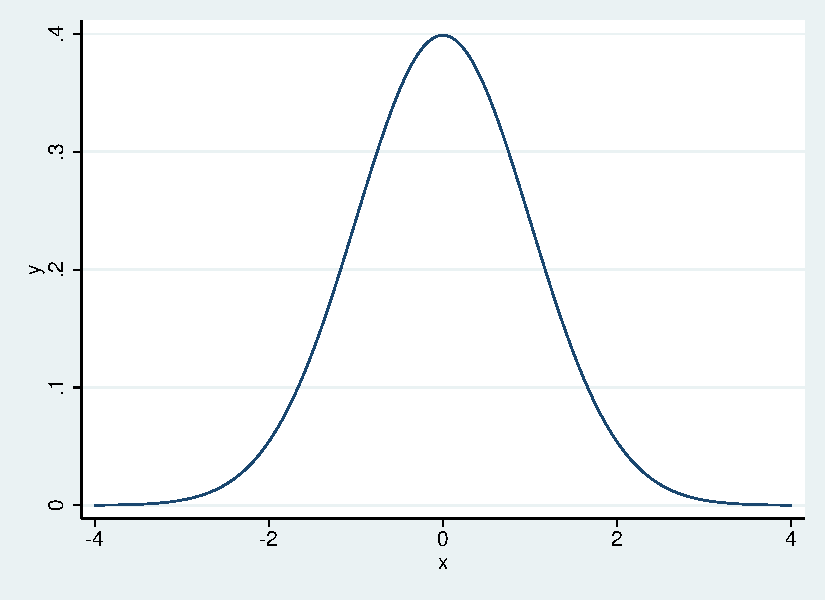
\includegraphics[width=0.33\textwidth]{mod3230.pdf}\\
Left graph is \lstinline{histogram} plot; the center is \lstinline{kdensity} plot; the right is \lstinline{function} plot.
\end{center}


\subsection{Graphics: Twoway Scatterplots}
This module shows some of the options when using the \lstinline{twoway} command to produce scatterplots.  This is illustrated by showing the command and the resulting graph.  This includes hotlinks to the \href{http://www.stata.com/help.cgi?graph}{Stata Graphics Manual} available over the web and from within Stata by typing \lstinline{help graph}.

\subsubsection{Two Way Scatterplots}
\textbf{Basic twoway scatterplot}
\begin{lstlisting}
twoway (scatter read write)
\end{lstlisting}
\begin{center}
\includegraphics[width=0.5\textwidth]{mod331.pdf}
\end{center}

\subsubsection{Schemes}
\begin{lstlisting}
twoway (scatter read write) , scheme(economist) // use the economist scheme (left)
twoway (scatter read write) , scheme(s1mono)    // use the s1mono scheme (right)
\end{lstlisting}
\begin{center}
\includegraphics[width=0.35\textwidth]{mod332.pdf}
\includegraphics[width=0.49\textwidth]{mod333.pdf}
\end{center}

\subsubsection{Marker Placement Options (i.e. Jitter)}
\begin{lstlisting}
twoway (scatter write read, jitter(3)) // with jitter option (left)
twoway (scatter write read)            // without jitter (right)
\end{lstlisting}
\begin{center}
\includegraphics[width=0.42\textwidth]{mod334.pdf}
\includegraphics[width=0.42\textwidth]{mod335.pdf}
\end{center}

\subsubsection{Marker Label Options}
\begin{lstlisting}
// Using small black square symbols.
twoway (scatter write read, msymbol(square) msize(small) mcolor(black))
// With markers red on the inside, black medium thick outline
twoway (scatter write read, mfcolor(red) mlcolor(black) mlwidth(medthick))
\end{lstlisting}
\begin{center}
\includegraphics[width=0.42\textwidth]{mod336.pdf}
\includegraphics[width=0.42\textwidth]{mod337.pdf}
\end{center}

\begin{lstlisting}
// Identifying Observations with Marker Labels
twoway (scatter read write, mlabel(id))
// Using large red marker labels at 12 O'clock
twoway (scatter read write if id <=10, mlabel(id) mlabposition(12) mlabsize(large) mlabcolor(red))
\end{lstlisting}
\begin{center}
\includegraphics[width=0.42\textwidth]{mod338.pdf}
\includegraphics[width=0.42\textwidth]{mod339.pdf}
\end{center}

\begin{lstlisting}
// Markers at 90 degree angle at 12 O'clock with a gap of 5
twoway (scatter read write if id <=10, mlabel(ses) mlabangle(90) mlabposition(12) mlabgap(5))
// If mlabgap option is omitted
twoway (scatter read write if id <=10, mlabel(ses) mlabangle(90) mlabposition(12))
\end{lstlisting}
\begin{center}
\includegraphics[width=0.42\textwidth]{mod3310.pdf}
\includegraphics[width=0.42\textwidth]{mod3311.pdf}
\end{center}


\begin{lstlisting}
// Modifying marker position separately for variables (1)
generate pos = 3
replace pos = 1 if (id == 5)
replace pos = 5 if (id == 6)
replace pos = 9 if (id == 3)
twoway (scatter read write if id <= 10, mlabel(ses) mlabv(pos))
// If option mlabv is not used
twoway (scatter read write if id <= 10, mlabel(ses))
\end{lstlisting}
\begin{center}
\includegraphics[width=0.40\textwidth]{mod3312.pdf}
\includegraphics[width=0.40\textwidth]{mod3313.pdf}
\end{center}

\subsubsection{Connect Options}

\begin{lstlisting}
// Connecting with straight line
egen mread = mean(read), by(write)
twoway (scatter mread write,connect(l) sort)
// If the sort option is omitted
twoway (scatter mread write,connect(l))
// Thick black dotted connecting line
twoway (scatter mread write,connect(l) clwidth(thick) clcolor(black) clpattern(dot) sort)
\end{lstlisting}
\begin{center}
\includegraphics[width=0.33\textwidth]{mod3314.pdf}
\includegraphics[width=0.33\textwidth]{mod3315.pdf}
\includegraphics[width=0.33\textwidth]{mod3316.pdf}
\end{center}


\begin{lstlisting}
// Show gaps in line when there are missing values
egen sdread = sd(read), by(write)
twoway (scatter sdread write, connect(l) sort cmissing(n))
// Omitting cmissing option
twoway (scatter sdread write, connect(l) sort)
\end{lstlisting}
\begin{center}
\includegraphics[width=0.40\textwidth]{mod3317.pdf}
\includegraphics[width=0.40\textwidth]{mod3318.pdf}
\end{center}

\subsection{Graphics: Combining Twoway Scatterplots}

This module shows examples of combining twoway scatterplots.  This is illustrated by showing the command and the resulting graph.  This includes hotlinks to the \href{http://www.stata.com/help.cgi?graph}{Stata Graphics Manual} available over the web and from within Stata by typing \lstinline{help graph}.

The data set used in these examples can be obtained using the following command:
\begin{lstlisting}
use "http://www.ats.ucla.edu/stat/stata/notes/hsb2.dta", clear
\end{lstlisting}

This illustrates combining graphs in the following situations.
\begin{compactitem}
\item Plots for separate groups (using \lstinline{by})
\item Combining separate plots together into a single plot
\item Combining separate graphs together into a single graph
\end{compactitem}

\subsubsection{Plots for separate groups}

\begin{lstlisting}
// Separate graphs by gender (male and female)
twoway (scatter read write), by(female)
// Separate graphs by ses and gender
twoway (scatter read write), by(female ses)
// Swapping position of ses and gender
twoway (scatter read write), by(ses female, cols(2))
\end{lstlisting}
\begin{center}
\includegraphics[width=0.33\textwidth]{mod341.pdf}
\includegraphics[width=0.33\textwidth]{mod342.pdf}
\includegraphics[width=0.33\textwidth]{mod343.pdf}
\end{center}

\subsubsection{Combining scatterplots and linear fit in one graph}

\begin{lstlisting}
// Scatterplot with linear fit
twoway (scatter read write) ///
       (lfit read write) ,
        ytitle(Reading Score)
// Graphs separated by SES and female with linear fit lines and points identified by id
twoway (scatter read write, mlabel(id)) ///
       (lfit read write, range(30 70)) ,
        ytitle(Reading Score) by(ses female)
// Graph for high ses females with linear fit with and without obs 51
twoway (scatter read write, mlabel(id)) ///
       (lfit read write, range(30 70)) ///
       (lfit read write if id != 51, range(30 70)) if female==1 & ses==3,
        ytitle(Reading Score) legend(lab(3 "Fitted values without Obs 51"))
\end{lstlisting}
\begin{center}
\includegraphics[width=0.33\textwidth]{mod344.pdf}
\includegraphics[width=0.33\textwidth]{mod345.pdf}
\includegraphics[width=0.33\textwidth]{mod346.pdf}
\end{center}

\subsubsection{Combining scatterplots with multiple variables and linear fits}

\begin{lstlisting}
// Reading and math score by writing score
twoway (scatter read write) ///        plot(1,1)
       (scatter math write)
// Reading and math score by writing score with fit lines
twoway (scatter read write) (scatter math write) /// plot(1,2)
       (lfit read write)    (lfit math write)    ///
// Adding legend to above graph
twoway (scatter read write) ///        plot(2,1)
       (scatter math write) ///
       (lfit read write)  ///
       (lfit math write), ///
       legend(label(3 "Linear Fit") label(4 "Linear Fit")) ///
       legend(order(1 3 2 4))
// Final version of graph making line style same as dot style, and ranges the same
twoway (scatter read write) ///        plot(2,2)
       (scatter math write) ///
       (lfit read write, pstyle(p1) range(25 80) )  ///
       (lfit math write, pstyle(p2) range(25 80) ), ///
       legend(label(3 "Linear Fit") label(4 "Linear Fit")) ///
       legend(order(1 3 2 4))
\end{lstlisting}
\begin{center}
\includegraphics[width=0.42\textwidth]{mod347.pdf}
\includegraphics[width=0.42\textwidth]{mod348.pdf}
\includegraphics[width=0.42\textwidth]{mod349.pdf}
\includegraphics[width=0.42\textwidth]{mod3410.pdf}
\end{center}


\subsubsection{Combining scatterplots and linear fit for separate groups}

\begin{lstlisting}
// Overlay graph of males and females in one graph
separate write, by(female)
twoway (scatter write0 read) (scatter write1 read), ///
       ytitle(Writing Score) legend(order(1 "Males" 2 "Females"))
// Overlay graph of males and females in one graph with linear fit lines
twoway (scatter write0 read) (scatter write1 read) ///
     (lfit write0 read) (lfit write1 read), ///
     ytitle(Writing Score) ///
     legend(order(1 "Males" 2 "Females" 3 "Lfit Males" 4 "Lfit Females"))
\end{lstlisting}
\begin{center}
\includegraphics[width=0.42\textwidth]{mod3411.pdf}
\includegraphics[width=0.42\textwidth]{mod3412.pdf}
\end{center}

\subsubsection{Combining separate graphs into one graph}
First, we make 3 graphs (not shown)
\begin{lstlisting}
// Making the Graphs
twoway (scatter read write) (lfit read write), name(scatterx)
regress read write
rvfplot, name(rvf)
lvr2plot, name(lvr)
\end{lstlisting}

Now we can use \lstinline{graph combine} to combine these into one graph, we can also move the place where the empty graph is located, as shown below.

\begin{lstlisting}
// Combine the three graphs into one graph
graph combine scatterx rvf lvr
// Combining the graphs differently
graph combine scatterx rvf lvr, hole(2)
\end{lstlisting}
\begin{center}
\includegraphics[width=0.42\textwidth]{mod3413.pdf}
\includegraphics[width=0.42\textwidth]{mod3414.pdf}
\end{center}

\subsection{Graphics: Common Graph Options}
This module shows examples of the different kinds of graphs that can be created with the \lstinline{graph twoway} command.  This is illustrated by showing the command and the resulting graph.  For more information, see the \href{http://www.stata.com/help.cgi?graph}{Stata Graphics Manual} available over the web and from within Stata by typing \lstinline{help graph}, and in particular the section on \textit{Two Way Scatterplots}.

\begin{lstlisting}
// Adding a title
graph twoway scatter read write, ///
  title("Scatterplot of Reading and Writing")
// Black title, positioned at 11 O'Clock
graph twoway scatter read write, ///
  title("Scatterplot of Reading and Writing", ///
  color(black) position(11))
// Title at 5 O'Clock, medium size text, positioned within the graph
graph twoway scatter read write, ///
  title("Scatterplot of Reading and Writing", ///
  size(medium) position(5) ring(0))
\end{lstlisting}
\begin{center}
\includegraphics[width=0.33\textwidth]{mod351.pdf}
\includegraphics[width=0.33\textwidth]{mod352.pdf}
\includegraphics[width=0.33\textwidth]{mod353.pdf}
\end{center}

\begin{lstlisting}
// Title in a box with cyan background, magenta border and a medium margin around the title
graph twoway scatter read write, ///
  title("Scatterplot of Reading and Writing", ///
         box bcolor(cyan) blcolor(magenta) bmargin(medium))
// Two line title with a gap of 3 between the titles
graph twoway scatter read write, ///
  title("Scatterplot of Reading and Writing" ///
  "Sample of 200 Students", linegap(3) )
\end{lstlisting}

\begin{center}
\includegraphics[width=0.42\textwidth]{mod354.pdf}
\includegraphics[width=0.42\textwidth]{mod355.pdf}
\end{center}

\begin{lstlisting}
// Graph with title, subtitle, caption, and a note
graph twoway scatter read write, ///
  title("Scatterplot of Reading and Writing") ///
  subtitle("Sample of 200 Students") ///
  note(High School and Beyond Data) ///
  caption(From www.ats.ucla.edu)
// Moving and sizing note and caption
graph twoway scatter read write, ///
  title("Scatterplot of Reading and Writing") ///
  subtitle("Sample of 200 Students") ///
  note(High School and Beyond Data, size(medium) position(5)) ///
  caption(From www.ats.ucla.edu, size(vsmall) position(5))
\end{lstlisting}

\begin{center}
\includegraphics[width=0.42\textwidth]{mod356.pdf}
\includegraphics[width=0.42\textwidth]{mod357.pdf}
\end{center}

\begin{lstlisting}
// Modifying title on x and y axis
twoway scatter read write, ///
  ytitle(Score on Writing Test) ///
  xtitle(Score on Reading Test)

// Complete example
twoway scatter read write, ///
  title("Scatterplot of Reading and Writing") ///
  subtitle("Sample of 200 Students") ///
  note(High School and Beyond Data, size(medium) position(5)) ///
  caption(From www.ats.ucla.edu, size(vsmall) position(5)) ///
  ytitle(Score on Writing Test) ///
  xtitle(Score on Reading Test)
\end{lstlisting}
\begin{center}
\includegraphics[width=0.42\textwidth]{mod358.pdf}
\includegraphics[width=0.42\textwidth]{mod359.pdf}
\end{center}

\begin{lstlisting}
// Sizing graph to have 4 by 2 aspect ratio
twoway scatter read write, ysize(2) xsize(4)

// Making text scaled 1.5 times normal size
graph twoway scatter read write, scale(1.5)
\end{lstlisting}

\begin{center}
\includegraphics[width=0.5\textwidth]{mod3510.pdf}
\includegraphics[width=0.42\textwidth]{mod3511.pdf}
\end{center}

\begin{lstlisting}
// Graph with sand color outside graph, gray inside graph
graph twoway scatter read write, ///
  title("Scatterplot of Reading and Writing") ///
  graphregion( color(sand) ) plotregion(  fcolor(gray) )

// Graph with sand color outside graph, gray inside graph, red outer border, blue inner border
graph twoway scatter read write, ///
  title("Scatterplot of Reading and Writing") ///
  graphregion( fcolor(red)  ifcolor(sand) ) ///
  plotregion(  fcolor(blue) ifcolor(gray))

// Graph with colors for many border elements
graph twoway scatter read write, ///
  title("Scatterplot of Reading and Writing") ///
  graphregion( fcolor(red)   lcolor(yellow)  lwidth(thick)  ///
              ifcolor(sand) ilcolor(orange)  ilwidth(thick)) ///
  plotregion(  fcolor(blue)  lcolor(green)   lwidth(thick)  ///
              ifcolor(gray) ilcolor(purple)  ilwidth(thick))
\end{lstlisting}

\begin{center}
\includegraphics[width=0.33\textwidth]{mod3512.pdf}
\includegraphics[width=0.33\textwidth]{mod3513.pdf}
\includegraphics[width=0.33\textwidth]{mod3514.pdf}
\end{center}
